\documentclass[xcolor=dvipsnames]{beamer}

\usepackage{amssymb,amsmath}
\usepackage[utf8]{inputenc}
\usepackage[russian]{babel}
\usepackage{amsthm}
\usepackage{amsfonts}
\usepackage{algorithmic, algorithm}
\usepackage{xcolor}
\usepackage{graphicx}
\graphicspath{ {images/} }

\newtheorem*{mynote}{Замечание}
\newtheorem{mydef}{Определение}
\newtheorem{mytheorem}{Теорема}
\newtheorem{statement}{Утверждение}
\newtheorem*{consequence}{Следствие}

\def \eval #1#2{\left.#1\right\vert_{#2}}
\def \<#1> {\langle #1 \rangle}
\def \n #1{\mathit{#1}}
\def \bigcupn {\bigcup\limits_{v=1}^{n}}
%Information to be included in the title page:
\title{Использование логических формул для кэширования универсальных запросов к Реляционной Базе Данных.}
\author{Мосин С.В.}
\institute{ИМ СО РАН (ОмФ)}
\date{2015}

\usetheme{Boadilla}
%\usecolortheme{seahorse}
\usefonttheme{serif}

\setbeameroption{hide notes}

\setbeamertemplate{note page}[plain]
\setbeamertemplate{theorems}[numbered]
\setbeamertemplate{footline}{%
    \raisebox{5pt}{\makebox[\paperwidth]{\hfill\makebox[20pt]{\color{gray}
          \scriptsize\insertframenumber}}}\hspace*{5pt}}
          
%\setbeamercolor*{frametitle}{bg=white, fg=brown}

\begin{document}
 
\frame{\titlepage}

\section{Клиент-серверная архитектура}

\begin{frame}
\frametitle{\insertsection}
\begin{center}
  \makebox[\textwidth]{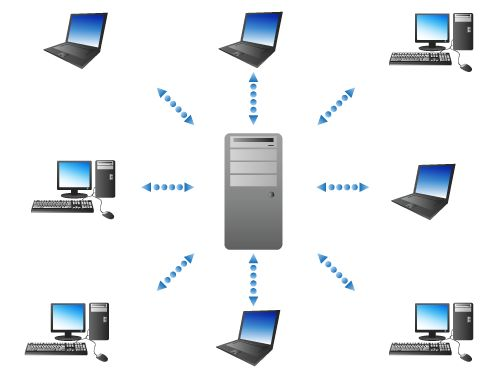
\includegraphics[width=0.6\paperwidth]{client-server}}
\end{center}
\end{frame}
\note{В данной работе рассматривается новый метод кэширования запросов к реляционной базе данных для
систем с центральным сервером и распределенными клиентами. Данные загружаются в клиентский кэш,
основываясь на запросах, выполненных на сервере БД.}
 %---------------------------------------------------------------------------------------%
 

\section{Пример использования кэша}

\begin{frame}
\frametitle{\insertsection}
Рассмотрим фрагмент схемы БД, представляющий учебный план в университете:
\vspace{\baselineskip}

$R_1 =\mbox{\it Студенты}\ (\mbox{\bf № студента}, \mbox{ФИО студента},
\mbox{Группа})$\\
$R_2 =\mbox{\it Расписание}\ (\mbox{\bf Группа}, \mbox{\bf № аудитории},
\mbox{Дисциплина})$\\
$R_3 =\mbox{\it Успеваемость}\ (\mbox{\bf № студента}, \mbox{\bf Дисциплина},
\mbox{Оценка})$
\note{На слайде фрагмент БД, где представлены 3 отношения. Имена отношений выделены курсивом, их
первичные ключи - жирным шрифтом.
Номер студента уникально определяет его имя и группу, у данной группы в конкретной аудитории
проходят занятия по данной конкретной дисциплине, а номер студента и дисциплина соответствуют одной
единственной оценке.}
\end{frame}

\begin{frame}
\frametitle{\insertsection}
\underline{Запрос 1}: Список студентов, изучающих физику, чей номер больше 210:
$$P_1 = \pi_{X_1}(\sigma_{F_1} (R_1 \Join R_2)),$$
где $\pi_{X_1}$ -- проекция по множеству атрибутов $X_1$
$X_1 = \{\text{№ студента},
\text{ФИО студента}, \text{Группа}, \text{Дисциплина}\}$,
$\sigma$ -- операция селекции,
$F_1$ -- логическая формула: $F_1 = (\text{№ студента} > 210\ \&\ \text{Дисциплина} =
\text{Физика})$, $\Join$ --операция естественного соедения.
\note{В результате данного запроса будут получены те кортежи БД, которые удовлетворяют формуле
$F_1$, причем с сервера будут запрошены только атрибуты $\text{№ студента},
\text{ФИО студента}, \text{Группа}, \text{Дисциплина}$}
\end{frame}


\begin{frame}
\frametitle{\insertsection}
\underline{Запрос 2}: Ведомости группы M10:
$$P_2 = \pi_{X_2}(\sigma_{F_2} (R_1 \Join R_3)),$$
где
$X_2 = \{\text{№ студента}, \text{Группа}, \text{Дисциплина}, \text{Оценка}\}$, $F_2$
-- логическая формула:\\
$F_2 = (\text{Группа}=\text{M10})$.
\note{Аналогично осуществляется Запрос 2, представляющий набор ведомостей по всем предметам для
студентов группы M10.}
\end{frame}


\begin{frame}
\frametitle{\insertsection}
$$P^{\ast} = \pi_{X^{\ast}}(\sigma_{F^{\ast}} (R_1 \Join R_2 \Join R_3 )),$$
где $X^{\ast}= \{\text{№ студента}, \text{Группа}, \text{Оценка}\}$, $F^{\ast}$
-- логическая формула: $F^{\ast} = (\textcolor<2>{blue}{\text{№ студента} > 300}\ \&\ 
\textcolor<3>{PineGreen}{\text{Группа} = \text{M10}}\ \&\ \textcolor<2>{brown}{\text{Дисциплина} = \text{Физика}})$.

\only<2>{$F_1 = (\textcolor{blue}{\text{№ студента} > 210}\ \&\ \textcolor{brown}{\text{Дисциплина} =
\text{Физика}})$}
\only<3>{$F_2 = (\textcolor{PineGreen}{\text{Группа}=\text{M10}})$.}

\vspace{\baselineskip}

\onslide<4>{Запрос может быть выполнен с использованием кэша:
$P^{\ast} =\pi_{X^{\ast}}(\sigma_{F_3} (P_1 \Join P_2 ))$, где $F_3$
-- логическая формула: $F_3 = (\text{Stud\_ID} > 300)$.}
\note<1>{Предположим теперь, что, пользователь хочет получить информацию, формализованную следующим
запросом (запрос $P^{\ast}$ на слайде). Это список оценок по физике студентов группы М10, чей номер больше 300.}
\note<4>{Сравнивая области истинности логических формул, используемых в $P_1$, $P_2$ и $P^{\ast}$,
получаем, что запрос может быть выполнен с помощью кэша.

Запрос к серверу в этом случае не требуется.}
\end{frame}
 %--------------------------------------------------------------------------------------- %


\section{Логические ограничения}

\begin{frame}
\frametitle{\insertsection}
Общий вид логической формулы:
\begin{equation}
F = K_1 \vee K_2 \vee \dots \vee K_m ,
\label{def_F_1}
\end{equation}
\begin{equation}
K_i = T_1 \&\ T_2 \dots \&\ T_n, i = 1, \dots, m ,
\label{def_F_2}
\end{equation}
здесь $T_j, j = 1, \dots, n$ - предикаты на множестве атрибутов БД
\end{frame}


\begin{frame}
\frametitle{\insertsection}
$\mathcal{A} =$ $\{(a_1, \dots, a_n) \mid a_i \in Dom(A_i), i=1,\dots,n\}$, где $Dom(A_i)$ -
множество всех допустимых значений атрибута $A_i$.

\vspace{\baselineskip}

$\mathcal{A} = Dom(A_1)\times Dom(A_2)\times \dots \times Dom(A_n)$ - $n$-мерное пространство
значений всех атрибутов базы данных. Текущее состояние базы данных соответствует подмножеству этого
пространства.

\note{Введем в рассмотрение множество $\mathcal{A}$.

Данное множество суть декартово произведение областей определения всех атрибутов, определенных в БД.

Допустимые состояния БД образуют лишь некоторую область в этом пространстве, соответствующую
ограничениям целостности на данные.}
\end{frame}


\begin{frame}
\frametitle{\insertsection}
\begin{mydef}
Областью истинности формулы $F$, определенной (\ref{def_F_1}),
(\ref{def_F_2}), называется множество $M (F) = \{a \in \mathcal{A} \mid
F(a) = \n {TRUE}\}$.
\end{mydef}

\onslide<2->
\begin{mydef}
Проекцией логической формулы $F$, определенной (\ref{def_F_1}), (\ref{def_F_2}) на множество
атрибутов $X$ называется логическая формула $F[X], \<F[X]> = X$, в
которой все предикаты $R_i^F.A_i^F \notin X$ заменены тривиальным предикатом $\n{TRUE}$.
\label{projection}
\end{mydef}

\note<1>{На данном слайде приведено понятие, на котором во многом основывается данная работа. Это
определение области истинности логической формулы.

На практике область истинности определяет все кортежи БД, которые удовлетворяют данной формуле, а
следовательно будут возвращены с сервера в ответ на пользовательский запрос. Однако обращаю внимание,
что в определении не используется конкретная реализация БД, а это значит, что области истинности
можно сравнивать аналитически, не осуществляя каких-либо запросов к серверу БД.}
\note<2>{Здесь приведено понятие проекции логической формулы, являющееся вспомогательным и необходимым
для формулировки дальнейших результатов.}
\end{frame}
 %---------------------------------------------------------------------------------------%
 
\section{Промежуточные представления данных}

\begin{frame}
\frametitle{\insertsection}
$P$=$\{ P_1$, $P_2$, $\dots$, $P_m \}$ - сохраненные промежуточные представления данных

\vspace{\baselineskip}

$$P_v = \pi_{X_v}(\sigma_{F_v} (R^v_1 \Join R^v_2 \Join \dots \Join R^v_{s(v)} ))$$\\
$s(v)$ – количество отношений БД, использованных при формировании $P_v$,\\
$\pi_{X_v}$ - операция проекции по множеству атрибутов $X_v$,\\
$\sigma_{F_v}$ - операция селекции с логическим ограничением на кортежи $F_v$.

\vspace{\baselineskip}

Целевое представление данных:
$$P^{\ast} = \pi_{X^{\ast}}(\sigma_{F^{\ast}} (R^{\ast}_1 \Join R^{\ast}_2\Join \dots \Join
R^{\ast}_l )$$

\note{Рассмотрим формализацию задачи. На входе имеем множество $P$ сохраненных в кеше запросов
пользователя.

Его элементы $P_v$ представлены в виде так называемых «универсальных запросов».
$(R^v_1, R^v_2, \dots, R^v_l )$ - некоторые отношения БД.
По сути это композиция операций естественного соединения, вырезки по строкам и по столбцам.
Большинство запросов на чтение к БД имеют в своей основе такой универсальный запрос.

Целевое представление данных, т.е. запрос пользователя, имеет такую же форму.
$(R^{\ast}_1, R^{\ast}_2, \dots, R^{\ast}_l )$ - некоторые вообще говоря другие отношения БД.}
\end{frame}


\begin{frame}
\frametitle{\insertsection}
\begin{mytheorem}
$P^{\ast} \subseteq \pi_{X^{\ast}} ( \sigma_{F^{\ast}[X]} (P_1 \Join \dots \Join
P_n))$, где $X = \bigcupn X_{v}$ если:
\\а) $X^{\ast} \subseteq X$
\\б)
$ \bigcupn \{R^{v}_{1}, \ldots, R^{v}_{s(v)}\} = \{R'_{1}, \ldots, R'_{s'}\}
\subseteq
\{R^{\ast}_{1}, \ldots, R^{\ast}_{l}\} $
\\в) $M(F^{\ast}) \subseteq M(F_{v}), v = 1,\dots,n $.
\label{th_mult}
\end{mytheorem}
\note{Предложенные в теореме условия гарантируют, что данные, необходимые для формирования представления $P^{\ast}$, содержатся в промежуточном представлении $P_v$. Однако в нем могут быть лишние кортежи, которые дают значение TRUE при подстановке в формулу $F^{\ast}$. Дело в том, что эти кортежи будут удалены при выполнении операции естественного соединения с отношениями, которых не хватает в множестве отношений $P_v$ для совпадения с множеством отношений $P^{\ast}$}
\end{frame}

\begin{frame}
\frametitle{\insertsection}
\begin{mytheorem}
$P^{\ast} =  \pi_{X^{\ast}} ( \sigma_{F^{\ast}} (P_1 \Join \dots \Join
P_n))$, где $X = \bigcupn X_{v}$ если:
\\а) $X^{\ast} \subseteq X$, $X_v \supseteq \<\Join_{i=1}^{s(v)} R^v_i> \cap (\bigcup\limits_{\substack{w=1\\ w \neq v}}^{n} \<\Join_{i=1}^{s(w)} R^w_i> ), v = 1,\dots,n$
\\б)
$ \bigcupn \{R^{v}_{1}, \ldots, R^{v}_{s(v)}\} = \{R'_{1}, \ldots, R'_{s'}\}
= \{R^{\ast}_{1}, \ldots, R^{\ast}_{l}\} $
\\в) $M(F^{\ast}) \subseteq M(F_{v}), v = 1,\dots,n $
\\г) $ \<F^{\ast}> \subseteq X $.
\label{th_mult_eq}
\end{mytheorem}

\note{Следующая теорема соответствует частному случаю, где проблема лишних кортежей не возникает.
Здесь добавляется условие на атрибуты формулы F, чтобы сделать возможным вырезку по строкам с
использованием самой формулы F, а не её проекции.

Первое условие сильно осложнилось для удовлетворения свойству операции проекции. Если этого не
потребовать, то могут появиться лишние данные при выполнении операций естественного соединения.

Остальные условия суть комбинация условий теорем 2 и 3.

Данная теорема является в некотором смысле ключевой, так как именно она позволяет на практике
воспользоваться содержимым кэша. Она применяется после проверки условий теорем 1 и 3.}
\end{frame}
 %---------------------------------------------------------------------------------------%
 
\section{Выводы}

\begin{frame}
\frametitle{\insertsection}
\begin{center}
\textbf{Что было сделано?}
\end{center}
\begin{itemize}
\item<2-> Подготовлена теоретическая база для разработки системы, взаимодействующей с БД
\end{itemize}
\note<2>{
Данный материал может быть использован для разработки ПО, являющегося прослойкой над СУБД и
управляющего использованием кэша, снижая тем самым количество передаваемых данных и общее время
работы системы.}

\onslide<3->
{
  \begin{center}
  \textbf{В чем отличие от существующих подходов?}
  \end{center}
}
\begin{itemize}
\item<4-> Использование семантики данных
\item<5-> \textbf{Аналитическая} проверка возможности использования кэша и определения
  недостающих данных
\end{itemize}
\note<4>{
Зарезервированные данные активно используется в системах управления базами данных (СУБД). Но в
большинстве случаев это касается повторного использования данных, записанных в кеш, без
предварительного анализа содержимого на предмет возможности частичного или комбинированного
использования.
}
\note<5>{Для осуществления проверки использования кэша анализируются области истинности логических
ограничений искомого запроса и запросов, результаты которых уже содержатся в кэше. 

Предложенный метод может быть использован для определения недостающих в кэше данных и
последующего запроса только на эти данные.

Для этого используются аналитические вычисления, что является принципиальным отличием данной работы от существующих технологий.
}

\onslide<6->
{
  \begin{center}
  \textbf{Что дальше?}
  \end{center}
}
\begin{itemize}
\item<7-> Актуализация данных
\item<8-> Динамическое формирование многомерных данных
\end{itemize}
\note<7>{Проблема актуализации данных не затрагивается в этой работе. Однако она может быть решена
путем учета запросов на сервере и обновлении данных при помощи триггеров.}
\note<8>{Предложенная технология будет использована при динамическом построении многомерных данных,
поскольку промежуточные представления имеют ту же структуру данных, что и таблицы соединений,
используемые для построения гиперкубов.}
\end{frame}
\end{document}